\chapter{AI: Algorithms}\label{AI: Algorithms}

\begin{customArrayStretch}{1.3}
\begin{table}[H]
\centering
\begin{tabular}{l c p{14.5cm}}

$V$ & set & set of vertices (nodes) of the graph \\

$E$ & set  & set of edges (links) of the graph \\

$b$ & $\in \mathbb{R}$ & \textbf{branching factor} or maximum number of successors of any node \\

$d$ & $\in \mathbb{R}$ & \textbf{depth} of the \textbf{shallowest goal} node (i.e., the number of steps along the path from the root) \\

$m$ & $\in \mathbb{R}$ & maximum length of any path in the state space \\

$\varepsilon$ & $\in \mathbb{R}$ & minimum step cost (small positive constant) \\

$C$ & $\in \mathbb{R}$ & cost of the solution \\

$C^\ast$ & $\in \mathbb{R}$ & cost of the optimal solution \\

$\ell$ & $\in \mathbb{R}$ & predetermined depth limit \\

$g(n)$ & $\in \mathbb{R}$ & Path Cost (The \textbf{actual cost} from the \textbfit{start node} to the current node $n$) (Eg: UCS) \\

$h(n)$ & $\in \mathbb{R}$ & Heuristic Estimate (The \textbf{estimated cost} from node $n$ to the \textbfit{goal}) (Eg: GBFS, A*) \\

$f(n)$ & $\in \mathbb{R}$ & Evaluation Function (The \textbf{total estimated cost} of the \textbfit{cheapest solution} through $n$) (Eg: A*) \\


\end{tabular}
\caption*{Notations}
\end{table}
\end{customArrayStretch}


\begin{enumerate}[itemsep=0.2cm]
    \item \textbf{heuristic function}
    \begin{enumerate}
        \item $h(n)$ = estimated cost of the cheapest path from the state at node $n$ to a goal state
        \hfill \cite{ai/book/Artificial-Intelligence-A-Modern-Approach/Russell-Norvig}

        \item Heuristic functions are the most common form in which additional knowledge of the problem is imparted to the search algorithm. 
        \hfill \cite{ai/book/Artificial-Intelligence-A-Modern-Approach/Russell-Norvig}
        
        \item if $n$ is a goal node, then $h(n)=0$
        \hfill \cite{ai/book/Artificial-Intelligence-A-Modern-Approach/Russell-Norvig}
    \end{enumerate}

    \item \textbf{evaluation function}:
    \begin{enumerate}
        \item The evaluation function $f$ is construed/ interpreted as a cost estimate, so the node with the lowest evaluation is expanded first.
        \hfill \cite{ai/book/Artificial-Intelligence-A-Modern-Approach/Russell-Norvig}
        
        \item The choice of $f$ determines the search strategy.
        \hfill \cite{ai/book/Artificial-Intelligence-A-Modern-Approach/Russell-Norvig}

        \item $f(n) = g(n)$ or $h(n)$ or $g(n)+h(n)$ or something else depending on the algorithm
    \end{enumerate}
\end{enumerate}





\section{Breadth-first search (BFS) \cite{ai/book/Artificial-Intelligence-A-Modern-Approach/Russell-Norvig}}
\label{AI: Algorithms/Breadth-first search (BFS)}


\begin{figure}[H]
    \centering
    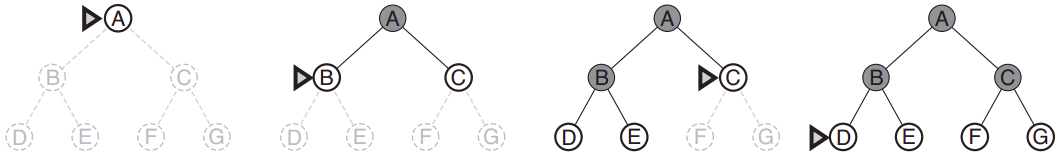
\includegraphics[
        width=\linewidth,
        height=4cm,
        keepaspectratio,
    ]{images/algorithms/Breadth-first-search-BT.png}
    \caption*{
        Breadth-first search on a simple binary tree. At each stage, the node to be expanded next is indicated by a marker.
        \cite{ai/book/Artificial-Intelligence-A-Modern-Approach/Russell-Norvig}
    }
\end{figure}


\begin{enumerate}[itemsep=0.2cm]
    \item Breadth-first search is a simple strategy in which the root node is expanded first, then all the successors of the root node are expanded next, then their successors, and so on. 
    \hfill \cite{ai/book/Artificial-Intelligence-A-Modern-Approach/Russell-Norvig}

    \item In general, all the nodes are expanded at a given depth in the search tree before any nodes at the next level are expanded.
    \hfill \cite{ai/book/Artificial-Intelligence-A-Modern-Approach/Russell-Norvig}

    \item Breadth-first search is an instance of the general graph-search algorithm in which the \textit{shallowest unexpanded node} is chosen for expansion.
    \hfill \cite{ai/book/Artificial-Intelligence-A-Modern-Approach/Russell-Norvig}

    \item new nodes (which are always deeper than their parents) go to the back of the queue, and old nodes, which are shallower than the new nodes, get expanded first. 
    \hfill \cite{ai/book/Artificial-Intelligence-A-Modern-Approach/Russell-Norvig}

    \item There is one slight tweak on the general graph-search algorithm, which is that the goal test is applied to each node when it is generated rather than when it is selected for expansion.
    \hfill \cite{ai/book/Artificial-Intelligence-A-Modern-Approach/Russell-Norvig}
    \\
    If the algorithm were to apply the goal test to nodes when selected for expansion, rather than when generated, the whole layer of nodes at depth d would be expanded before the goal was detected and the time complexity would be $\mathcal{O}(b\ ^{d+1})$.
    \hfill \cite{ai/book/Artificial-Intelligence-A-Modern-Approach/Russell-Norvig}

    \item the algorithm, following the general template for graph search, discards any new path to a state already in the frontier or explored set; it is easy to see that any such path must be at least as deep as the one already found. 
    \hfill \cite{ai/book/Artificial-Intelligence-A-Modern-Approach/Russell-Norvig}

    \item breadth-first search \textbf{always} has the \textit{shallowest path} to every node on the frontier. 
    As soon as a goal node is generated, we know it is the shallowest goal node because all shallower nodes must have been generated already and failed the goal test. 
    \hfill \cite{ai/book/Artificial-Intelligence-A-Modern-Approach/Russell-Norvig}

    \item \textbf{performance}:
    \begin{enumerate}[itemsep=0.2cm]
        \item \textbf{complete}: if the shallowest goal node is at some finite depth $d$, breadth-first search will eventually find it after generating all shallower nodes (provided the branching factor $b$ is finite). 
        \hfill \cite{ai/book/Artificial-Intelligence-A-Modern-Approach/Russell-Norvig}

        \item  the shallowest goal node is \textbf{not necessarily} the \textit{optimal} one. 
        breadth-first search is optimal if the path cost is a non-decreasing function of the depth of the node.
        The most common such scenario is that all actions have the same cost.
        the algorithm is optimal if step costs are all identical.
        \hfill \cite{ai/book/Artificial-Intelligence-A-Modern-Approach/Russell-Norvig}

        \item \textbf{Space Complexity}:
        \begin{enumerate}[itemsep=0.1cm]
            \item explored set: $\mathcal{O}(b\ ^{d-1})$
            \hfill \cite{ai/book/Artificial-Intelligence-A-Modern-Approach/Russell-Norvig}

            \item frontier: $\mathcal{O}(b\ ^{d})$
            \hfill \cite{ai/book/Artificial-Intelligence-A-Modern-Approach/Russell-Norvig}

            \item overall: $\mathcal{O}(b\ ^{d})$
            \hfill \cite{ai/book/Artificial-Intelligence-A-Modern-Approach/Russell-Norvig}
        \end{enumerate}

        \item \textbf{Time Complexity}: 
        $\mathcal{O}(b\ ^{d})$
        \hfill \cite{ai/book/Artificial-Intelligence-A-Modern-Approach/Russell-Norvig}

    \end{enumerate}

    \item \textbf{Disadvantages}:
    \begin{enumerate}[itemsep=0.1cm]
        \item the memory requirements are a bigger problem for breadth-first search than is the execution time.
        \hfill \cite{ai/book/Artificial-Intelligence-A-Modern-Approach/Russell-Norvig}

        
    \end{enumerate}

\end{enumerate}


\subsection*{Implementation}

\begin{enumerate}
    \item \textbf{frontier}: FIFO queue
\end{enumerate}


\vspace{0.5cm}


\begin{algorithm}[H]
    \caption{Breadth-first search on a graph. \cite{ai/book/Artificial-Intelligence-A-Modern-Approach/Russell-Norvig}}

    \SetKwFunction{FUNCTION}{\textsc{Breadth-First-Search}}
    \SetKwProg{Fn}{function}{ returns \normalfont{a solution, or failure}}{end}
    \Fn{\FUNCTION{problem}}{
        $node \ \gets$ a node with \textsc{State} = $problem$.\textsc{Initial-State}, \textsc{Path-Cost} = $0$ \\
        \ \\
        \If{$problem$.\textsc{Goal-Test}($node$.\textsc{State})}{
            \Return \textsc{Solution}($node$)
        }
        \ \\
        $frontier \ \gets$ a FIFO queue with node as the only element \\
        $explored \ \gets$ an empty set \\
        \ \\
        \While{}{
            \If{\textsc{Empty?}($frontier$)}{
                \Return failure
            }
            \ \\
            \Comment{chooses the shallowest node in $frontier$}
            $node \ \gets$ \textsc{Pop}($frontier$) \\ 
            add $node$.\textsc{State} to $explored$ \\
            \ \\
            \ForEach{$action$ \textbf{in} $problem$.\textsc{Actions}($node$.\textsc{State})}{
                $child \gets$ \textsc{Child-Node}($problem,\ node,\ action$) \\
                \If{$child$.\textsc{State} is \textbf{not in} $explored$ or $frontier$}{
                    \If{$problem$.\textsc{Goal-Test}($child$.\textsc{State})}{
                        \Return \textsc{Solution}($child$)
                    }
                    $frontier \gets$ \textsc{Insert}($child,\ frontier$)
                }
            }
        }
    }
\end{algorithm}


\begin{lstlisting}[
    language=Python,
    caption=Problem Solving Agent - Breadth-first search on a graph
]
from queue import Queue

def breadth_first_search(problem: Problem):
    node = Node(problem.initial_state, None, None, 0)

    if problem.goal_test(node.state):
        return solution(node)
    
    frontier = Queue()
    explored = set()

    frontier.put(node)

    while True:
        if frontier.empty():
            return None
        
        node = frontier.get()
        explored.add(node)

        for action in problem.actions(node.state):
            child = child_node(problem, node, action)
            
            if (not any([n.state == child.state for n in frontier.queue]) and 
                not any([n.state == child.state for n in explored])):
                if problem.goal_test(child.state):            
                    return solution(child)

                frontier.put(child)
\end{lstlisting}












\section{Uniform-cost search (UCS) \cite{ai/book/Artificial-Intelligence-A-Modern-Approach/Russell-Norvig}}
\label{AI: Algorithms/Uniform-cost search (UCS)}


\begin{enumerate}[itemsep=0.2cm]
    \item Instead of expanding the shallowest node (as in BFS), uniform-cost search expands the node $n$ with the \textbfit{lowest path cost} $g(n)$.
    \hfill \cite{ai/book/Artificial-Intelligence-A-Modern-Approach/Russell-Norvig}

    \item \textbf{Performance}:
    \begin{enumerate}[itemsep=0.2cm]
        \item uniform-cost search is \textbf{optimal} in general. 
        uniform-cost search expands nodes in order of their optimal path cost.
        \hfill \cite{ai/book/Artificial-Intelligence-A-Modern-Approach/Russell-Norvig}

        \item \textbf{Completeness is guaranteed} provided the cost of every step exceeds some small positive constant $\varepsilon$ and $b$ is finite
        \hfill \cite{ai/book/Artificial-Intelligence-A-Modern-Approach/Russell-Norvig}

        \item \textbf{Space Complexity}:
        \begin{enumerate}[itemsep=0.2cm]
            \item worst: $\mathcal{O}(b^{1 + \dfloor{C^\ast / \varepsilon}})$
            \hfill (can be much greater than $b^d$)
            \hfill \cite{ai/book/Artificial-Intelligence-A-Modern-Approach/Russell-Norvig}

            \item When all step costs are equal: $\mathcal{O}(b^{\ d+1})$
            \hfill \cite{ai/book/Artificial-Intelligence-A-Modern-Approach/Russell-Norvig}
        \end{enumerate}

        \item \textbf{Time Complexity}:
        \begin{enumerate}[itemsep=0.2cm]
            \item worst: $\mathcal{O}(b^{1 + \dfloor{C^\ast / \varepsilon}})$
            \hfill (can be much greater than $b^d$)
            \hfill \cite{ai/book/Artificial-Intelligence-A-Modern-Approach/Russell-Norvig}

            \item When all step costs are equal: $\mathcal{O}(b^{\ d+1})$
            \hfill \cite{ai/book/Artificial-Intelligence-A-Modern-Approach/Russell-Norvig}
        \end{enumerate}
    \end{enumerate}

    \item \textbf{Disadvantages}:
    \begin{enumerate}[itemsep=0.2cm]
        \item it will get stuck in an \textbf{infinite loop} if there is a path with an infinite sequence of \textit{zero-cost actions} - for example, a sequence of $NoOp$ actions.
        \hfill \cite{ai/book/Artificial-Intelligence-A-Modern-Approach/Russell-Norvig}

        \item  it suffers from the same difficulties with realvalued costs
        \hfill \cite{ai/book/Artificial-Intelligence-A-Modern-Approach/Russell-Norvig}
    \end{enumerate}

    \item When all step costs are the same, uniform-cost search is similar to breadth-first search, except that the latter stops as soon as it generates a goal, whereas uniform-cost search examines all the nodes at the goal’s depth to see if one has a lower cost; thus uniform-cost search does strictly more work by expanding nodes at depth $d$ unnecessarily.
    \hfill \cite{ai/book/Artificial-Intelligence-A-Modern-Approach/Russell-Norvig}
\end{enumerate}




\subsection*{Implementation}

\begin{enumerate}
    \item  This is done by storing the frontier as a \textbf{priority queue} ordered by $g(n)$. 
    \hfill \cite{ai/book/Artificial-Intelligence-A-Modern-Approach/Russell-Norvig}

    \item In addition to the ordering of the queue by path cost, there are two other significant differences from breadth-first search.
    \hfill \cite{ai/book/Artificial-Intelligence-A-Modern-Approach/Russell-Norvig}
    \begin{enumerate}
        \item  goal test is applied to a node when it is \textit{selected for expansion} rather than when it is first generated.
        The reason is that the first goal node that is \textit{generated} may be on a suboptimal path.
        \hfill \cite{ai/book/Artificial-Intelligence-A-Modern-Approach/Russell-Norvig}

        \item a test is added in case a better path is found to a node currently on the frontier.
        \hfill \cite{ai/book/Artificial-Intelligence-A-Modern-Approach/Russell-Norvig}
    \end{enumerate}

\end{enumerate}

\vspace{0.5cm}


\begin{algorithm}[H]
    \caption{\textsc{Uniform-Cost} search on a graph. \cite{ai/book/Artificial-Intelligence-A-Modern-Approach/Russell-Norvig}}

    \SetKwFunction{FUNCTION}{\textsc{Uniform-Cost-Search}}
    \SetKwProg{Fn}{function}{ returns \normalfont{a solution, or failure}}{end}
    \Fn{\FUNCTION{problem}}{
        $node \ \gets$ a node with \textsc{State} = $problem$.\textsc{Initial-State}, \textsc{Path-Cost} = $0$ \\
        $frontier \ \gets$ a \textbfit{priority queue} ordered by \textsc{Path-Cost}, with $node$ as the only element \\
        $explored \ \gets$ an empty set \\
        \ \\
        \While{}{
            \lIf{\textsc{Empty?}($frontier$)}{
                \Return failure
            }
            \Comment{chooses the lowest-cost node in $frontier$}
            $node \ \gets$ \textsc{Pop}($frontier$) \\ 
            \lIf{$problem$.\textsc{Goal-Test}($node$.\textsc{State})}{
                \Return \textsc{Solution}($node$)
            }
            add $node$.\textsc{State} to $explored$ \\
            \ \\
            \ForEach{$action$ \textbf{in} $problem$.\textsc{Actions}($node$.\textsc{State})}{
                $child \gets$ \textsc{Child-Node}($problem,\ node,\ action$) \\
                \If{\normalfont $child$.\textsc{State} is not in $explored$ or $frontier$}{
                    $frontier \gets$ \textsc{Insert}($child,\ frontier$)
                }
                \ElseIf{\normalfont $child$.\textsc{State} is in $frontier$ with higher \textsc{Path-Cost}}{
                    replace that $frontier$ node with $child$
                }
            }
        }
    }
\end{algorithm}


\begin{lstlisting}[
    language=Python,
    caption=Problem Solving Agent - Uniform cost search on a graph
]
import heapq

def uniform_cost_search(problem: Problem):
    node = Node(problem.initial_state, None, None, 0)

    if problem.goal_test(node.state):
        return solution(node)
    
    frontier = [(node.path_cost, node)]
    explored = set()

    heapq.heapify(frontier)

    while True:
        if len(frontier) == 0:
            return None
        
        path_cost, node = frontier.pop(0)

        if problem.goal_test(node.state):
            return solution(node)

        explored.add(node)
        for action in problem.actions(node.state):
            child = child_node(problem, node, action)

            if (not any([n.state == child.state for (path_cost, n) in frontier])
                and not any([n.state == child.state for n in explored])):
                frontier.append((child.path_cost, child))
                heapq.heapify(frontier)
            else:
                for idx, (path_cost, n) in enumerate(frontier):
                    if n.state == child.state and path_cost > child.path_cost:
                        frontier[idx] = (child.path_cost, child)
                        heapq.heapify(frontier)
\end{lstlisting}






\section{Depth-first search (DFS) \cite{ai/book/Artificial-Intelligence-A-Modern-Approach/Russell-Norvig}}


\begin{figure}[H]
\centering
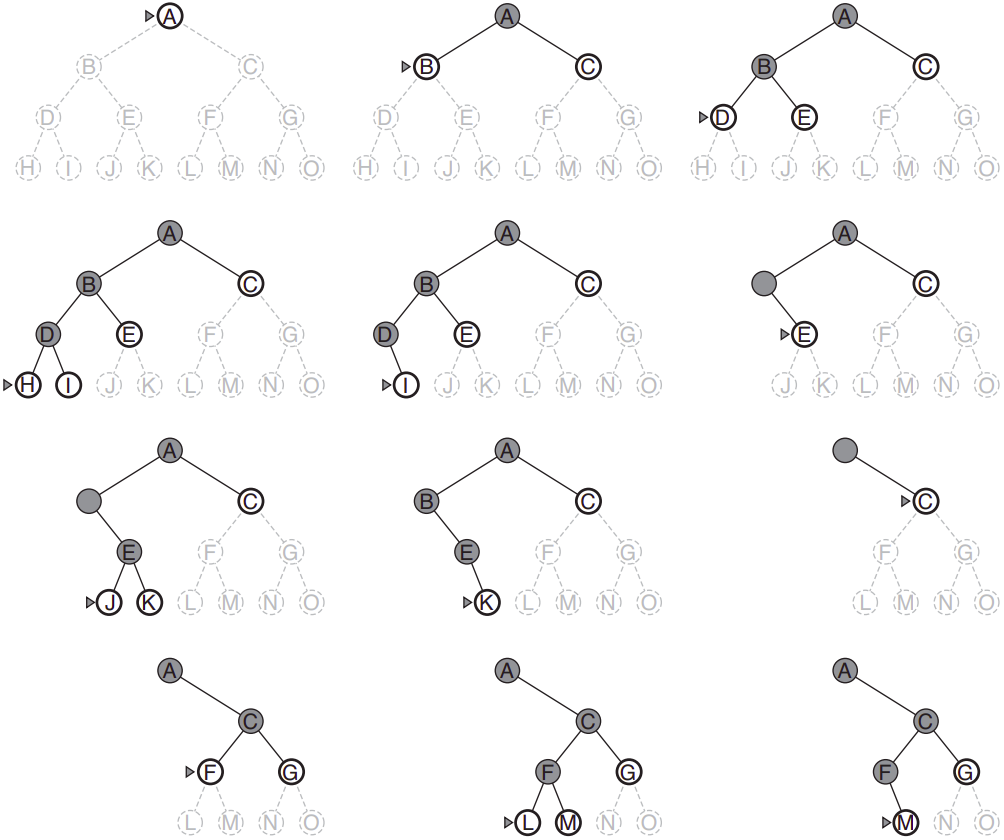
\includegraphics[
    width=\linewidth,
    height=7cm,
    keepaspectratio,
]{images/algorithms/Depth-first-search-illustration.png}
\caption*{
    Depth-first search on a binary tree. The unexplored region is shown in light gray. Explored nodes with no descendants in the frontier are removed from memory. Nodes at depth $3$ have no successors and $M$ is the only goal node. 
    \cite{ai/book/Artificial-Intelligence-A-Modern-Approach/Russell-Norvig}
}
\end{figure}


\begin{enumerate}[itemsep=0.2cm]
    \item Depth-first search always expands the \textbf{deepest node} in the current frontier of the search tree.
    \hfill \cite{ai/book/Artificial-Intelligence-A-Modern-Approach/Russell-Norvig}

    \item The search proceeds immediately to the deepest level of the search tree, where the nodes have no successors. As those nodes are expanded, they are dropped from the frontier, so then the search “backs up” to the next deepest node that still has unexplored successors.
    \hfill \cite{ai/book/Artificial-Intelligence-A-Modern-Approach/Russell-Norvig}

    \item \textbf{Performance}:
    \begin{enumerate}[itemsep=0.2cm]
        \item \textbf{graph-search version}:
        \begin{enumerate}[itemsep=0.2cm]
            \item \textbf{complete} in finite state spaces because it will eventually expand every node
            \hfill \cite{ai/book/Artificial-Intelligence-A-Modern-Approach/Russell-Norvig}

            \item \textbf{not optimal}
            \hfill \cite{ai/book/Artificial-Intelligence-A-Modern-Approach/Russell-Norvig}

            \item \textbf{time complexity}: $\mathcal{O}(b^d)$
            \hfill \cite{ai/book/Artificial-Intelligence-A-Modern-Approach/Russell-Norvig}

            \item \textbf{space complexity}: $\mathcal{O}(b^d)$
            \hfill \cite{ai/book/Artificial-Intelligence-A-Modern-Approach/Russell-Norvig}
        \end{enumerate}

        \item \textbf{tree-search version}:
        \begin{enumerate}[itemsep=0.2cm]
            \item \textbf{not complete}, as it can fall in \textit{infinite loop}
            \hfill \cite{ai/book/Artificial-Intelligence-A-Modern-Approach/Russell-Norvig}

            \item \textbf{not optimal}
            \hfill \cite{ai/book/Artificial-Intelligence-A-Modern-Approach/Russell-Norvig}

            \item \textbf{time complexity}: $\mathcal{O}(b^m)$
            \hfill \cite{ai/book/Artificial-Intelligence-A-Modern-Approach/Russell-Norvig}

            \item \textbf{space complexity}: $\mathcal{O}(b\ m)$
            \hfill \cite{ai/book/Artificial-Intelligence-A-Modern-Approach/Russell-Norvig}
        \end{enumerate}
    \end{enumerate}
\end{enumerate}


\subsection{Implementation}

\begin{enumerate}[itemsep=0.2cm]
    \item The depth-first search algorithm is an instance of the graph-search algorithm that uses a LIFO queue.
    \hfill \cite{ai/book/Artificial-Intelligence-A-Modern-Approach/Russell-Norvig}

    \item  it is common to implement depth-first search with a recursive function that calls itself  on each of its children in turn. 
    \hfill \cite{ai/book/Artificial-Intelligence-A-Modern-Approach/Russell-Norvig}
\end{enumerate}

\begin{lstlisting}[
    language=Python,
    caption=Problem Solving Agent - Depth first search on a graph
]
from queue import LifoQueue

def depth_first_search(problem: Problem):
    node = Node(problem.initial_state, None, None, 0)

    if problem.goal_test(node.state):
        return solution(node)
    
    frontier = LifoQueue()
    explored = set()

    frontier.put(node)

    while True:
        if frontier.empty():
            return None
        
        node = frontier.get()
        explored.add(node)

        for action in problem.actions(node.state):
            child = child_node(problem, node, action)

            if (not any([n.state == child.state for n in frontier.queue]) and 
                not any([n.state == child.state for n in explored])):
                if problem.goal_test(child.state):
                    return solution(child)

                frontier.put(child)
\end{lstlisting}















\section{Backtracking Search \cite{ai/book/Artificial-Intelligence-A-Modern-Approach/Russell-Norvig}}
\label{AI: Algorithms/Backtracking Search}


\begin{enumerate}
    \item A variant of depth-first search that uses still less memory.
    \hfill \cite{ai/book/Artificial-Intelligence-A-Modern-Approach/Russell-Norvig}

    \item \textbf{only one successor} is generated at a time rather than all successors; each partially expanded node remembers which successor to generate next.
    \hfill \cite{ai/book/Artificial-Intelligence-A-Modern-Approach/Russell-Norvig}

    \item \textbf{Performance}:
    \begin{enumerate}
        \item \textbf{Space Complexity}: $\mathcal{O}(m)$
        \hfill \cite{ai/book/Artificial-Intelligence-A-Modern-Approach/Russell-Norvig}
    \end{enumerate}

    \item \textbf{Advantages}:
    \begin{enumerate}
        \item  Backtracking search facilitates memory-saving (and time-saving) trick: the idea of generating a successor by \textbf{modifying} the current state description directly rather than copying it first.
        For this to work, we must be able to \textbf{undo} each modification when we go back to generate the next successor.
        \hfill \cite{ai/book/Artificial-Intelligence-A-Modern-Approach/Russell-Norvig}

        \item For problems with large state descriptions, such as robotic assembly, these techniques are critical to success.
        \hfill \cite{ai/book/Artificial-Intelligence-A-Modern-Approach/Russell-Norvig}
    \end{enumerate}
\end{enumerate}



\begin{lstlisting}[
    language=Python,
    caption=Problem Solving Agent - Backtracking using recursion \cite{common/online/chatgpt}
]
def backtrack(node: Node, explored: set):
    if problem.goal_test(node.state):
        return solution(node)

    explored.add(node)

    for action in problem.actions(node.state):
        child = child_node(problem, node, action)
        if not any([child.state == n.state for n in explored]):
            result = backtrack(child, explored)
            if result is not None:
                return result

    # Optional: allow revisiting for other paths (depends on problem)
    explored.remove(node)
    return None

def backtracking_search(problem: Problem):
    root = Node(problem.initial_state, None, None, 0)
    return backtrack(root, set())
\end{lstlisting}















\section{Depth-limited search \cite{ai/book/Artificial-Intelligence-A-Modern-Approach/Russell-Norvig}}

\begin{enumerate}[itemsep=0.2cm]
    \item The embarrassing failure of depth-first search in infinite state spaces can be alleviated by supplying depth-first search with a predetermined depth limit $\ell$. That is, nodes at depth  $\ell$ are treated as if they have no successors. 
    \hfill \cite{ai/book/Artificial-Intelligence-A-Modern-Approach/Russell-Norvig}

    \item \textbf{Performance}:
    \begin{enumerate}
        \item \textbf{Completeness}: NO \textbf{if} $\ell < d$ \textbf{else} YES
        \hfill \cite{ai/book/Artificial-Intelligence-A-Modern-Approach/Russell-Norvig}

        \item \textbf{Optimal}: NO \textbf{if} $\ell > d$ \textbf{else} YES
        \hfill \cite{ai/book/Artificial-Intelligence-A-Modern-Approach/Russell-Norvig}

        \item \textbf{time complexity}: $\mathcal{O}(b^\ell)$
        \hfill \cite{ai/book/Artificial-Intelligence-A-Modern-Approach/Russell-Norvig}

        \item \textbf{space complexity}: $\mathcal{O}(b\ell)$
        \hfill \cite{ai/book/Artificial-Intelligence-A-Modern-Approach/Russell-Norvig}
    \end{enumerate}

    \item Depth-first search can be viewed as a special case of depth-limited search with $\ell = \infty$.
    \hfill \cite{ai/book/Artificial-Intelligence-A-Modern-Approach/Russell-Norvig}

    \item diameter of the state space can be a better limit for efficiency
    \hfill \cite{ai/book/Artificial-Intelligence-A-Modern-Approach/Russell-Norvig}

    
\end{enumerate}


\vspace{0.5cm}

\begin{algorithm}[H]
    \caption{A recursive implementation of depth-limited tree search. \cite{ai/book/Artificial-Intelligence-A-Modern-Approach/Russell-Norvig}}


    \SetKwFunction{FUNCTION}{\textsc{Depth-Limited-Search}}
    \SetKwProg{Fn}{function}{ returns \normalfont{a solution, or failure/cutoff}}{end}
    \Fn{\FUNCTION{problem, limit}}{
        \Return \textsc{Recursive-DLS}( \\
            \hspace{0.5cm}  \textsc{Make-Node}($problem$.\textsc{Initial-State}), \\
            \hspace{0.5cm}  $problem$, \\
            \hspace{0.5cm}  $limit$, \\
        )
    }
    
    \ \\
    
    \SetKwFunction{FUNCTION}{\textsc{Recursive-DLS}}
    \SetKwProg{Fn}{function}{ returns \normalfont{a solution, or failure/cutoff}}{end}
    \Fn{\FUNCTION{node, problem, limit}}{
        \If{\normalfont $problem$.\textsc{Goal-Test}($node$.\textsc{State})}{
            \Return \textsc{Solution}($node$) 
        }
        \ElseIf{limit = 0}{
            \Return $cutoff$
        }
        \Else{
            $cutoff\_occurred? \ \gets$ false\\
            \ \\
            \ForEach{\normalfont $action$ \textbf{in} $problem$.\textsc{Actions}($node$.\textsc{State})}{
                $child \gets$ \textsc{Child-Node}($problem,\ node,\ action$)\\
                $result \gets$ \textsc{Recursive-DLS}($child,\ problem,\ limit-1$)\\
                \If{result = cutoff}{
                    $cutoff\_occurred? \ \gets$ true
                }
                \ElseIf{result $\neq$ failure}{
                    \Return $result$
                }
            }
            \ \\
            \If{$cutoff\_occurred?$}{
                \Return $cutoff$
            }
            \Else{
                \Return $failure$
            }
        }
    }
\end{algorithm}


\begin{lstlisting}[
    language=Python,
    caption=Problem Solving Agent - Depth limited search (recursive)
]
CUTOFF = "CUT-OFF"

def depth_limited_search(problem: Problem, limit: int):
    return recursive_dls(
        Node(problem.initial_state, None, None, 0),
        problem,
        limit,
    )

def recursive_dls(node: Node, problem: Problem, limit: int):
    if problem.goal_test(node.state):
        return solution(node)
    
    elif limit == 0:
        return CUTOFF
    
    else:
        cutoff_occurred = False
        for action in problem.actions(node.state):
            child = child_node(problem, node, action)
            result = recursive_dls(child, problem, limit-1)
            if result == CUTOFF:
                cutoff_occurred = True
            elif result is not None:
                return result
        if cutoff_occurred:
            return CUTOFF
        else:
            return
\end{lstlisting}


\vspace{0.5cm}

\begin{enumerate}[itemsep=0.2cm]
    \item $failure$ value indicates no solution
    \hfill \cite{ai/book/Artificial-Intelligence-A-Modern-Approach/Russell-Norvig}

    \item $cutoff$ value indicates no solution within the depth limit
    \hfill \cite{ai/book/Artificial-Intelligence-A-Modern-Approach/Russell-Norvig}
\end{enumerate}








\section{Iterative Deepening Search (IDS) \cite{ai/book/Artificial-Intelligence-A-Modern-Approach/Russell-Norvig}}
\label{AI: Algorithms/Iterative Deepening Search (IDS)}


\begin{figure}[h!]
    \centering
    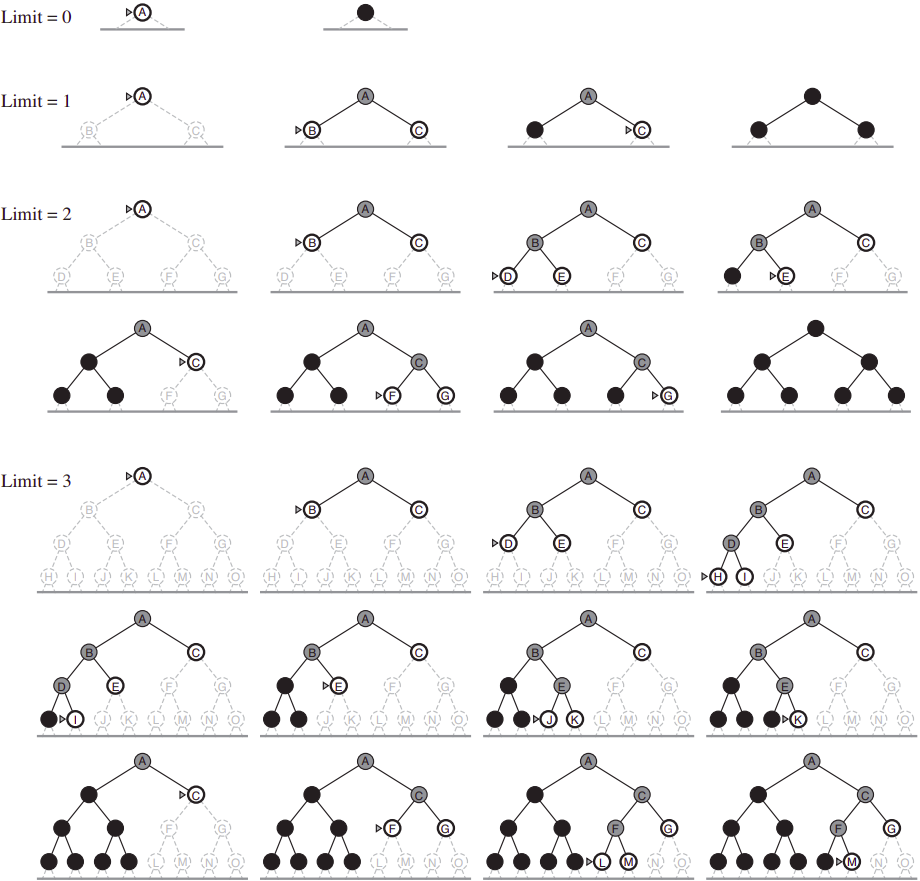
\includegraphics[
        width=\linewidth,
        height=14cm,
        keepaspectratio,
    ]{images/algorithms/iterative-deepening-search-BT.png}
    \caption*{Four iterations of iterative deepening search on a binary tree \cite{ai/book/Artificial-Intelligence-A-Modern-Approach/Russell-Norvig}}
\end{figure}


\begin{enumerate}
    \item \textbf{Iterative deepening search} (or \textbf{iterative deepening depth-first search}) is a general strategy, often used in combination with depth-first tree search, that finds the best depth limit.
    \hfill \cite{ai/book/Artificial-Intelligence-A-Modern-Approach/Russell-Norvig}

    \item It gradually increases the depth limit $\ell \in \dCurlyBrac{0,1,2,\cdots,\infty}$ till a goal is found, which occurs when $\ell = d$ ($d$ is unknown in reality)
    \hfill \cite{ai/book/Artificial-Intelligence-A-Modern-Approach/Russell-Norvig}

    \item Iterative deepening combines the benefits of depth-first and breadth-first search.
    \hfill \cite{ai/book/Artificial-Intelligence-A-Modern-Approach/Russell-Norvig}
    \begin{enumerate}
        \item Like depth-first search, its memory requirements are modest: $\mathcal{O}(b d)$ to be precise. 
        \hfill \cite{ai/book/Artificial-Intelligence-A-Modern-Approach/Russell-Norvig}

        \item Like breadth-first search, it is complete when the branching factor is finite and optimal when the path cost is a non-decreasing function of the depth of the node.
        \hfill \cite{ai/book/Artificial-Intelligence-A-Modern-Approach/Russell-Norvig}
    \end{enumerate}

    \item total number of nodes generated in the worst case is
    \\
    $N(\text{IDS})=(d)b + (d - 1)b^2 + \cdots + (1)b^d$
    \hfill \cite{ai/book/Artificial-Intelligence-A-Modern-Approach/Russell-Norvig}

    \item you can use a hybrid approach that runs breadth-first search until almost all the available memory is consumed, and then runs iterative deepening from all the nodes in the frontier.
    \hfill \cite{ai/book/Artificial-Intelligence-A-Modern-Approach/Russell-Norvig}

    \item iterative deepening is the \textit{preferred uninformed search} method when the search space is large and the depth of the solution is not known.
    \hfill \cite{ai/book/Artificial-Intelligence-A-Modern-Approach/Russell-Norvig}

    \item \textbf{Performance}:
    \begin{enumerate}
        \item \textbf{completeness}: YES \textbf{if} $b$ is finite \textbf{else} NO
        \hfill \cite{ai/book/Artificial-Intelligence-A-Modern-Approach/Russell-Norvig}

        \item \textbf{optimal}: YES \textbf{if} path cost is a non-deceasing function of depth of the node \textbf{else} NO
        \hfill \cite{ai/book/Artificial-Intelligence-A-Modern-Approach/Russell-Norvig}
        
        \item \textbf{space complexity}: $\mathcal{O}(b d)$
        \hfill \cite{ai/book/Artificial-Intelligence-A-Modern-Approach/Russell-Norvig}

        \item \textbf{time complexity}: $\mathcal{O}(b^d)$
        \hfill \cite{ai/book/Artificial-Intelligence-A-Modern-Approach/Russell-Norvig}
    \end{enumerate}
\end{enumerate}

\vspace{0.5cm}

\begin{algorithm}[H]
    \caption{The iterative deepening search algorithm, which repeatedly applies depth-limited search with increasing limits. It terminates when a solution is found or if the depth-limited search returns failure, meaning that no solution exists. \cite{ai/book/Artificial-Intelligence-A-Modern-Approach/Russell-Norvig}}

    \SetKwFunction{FUNCTION}{\textsc{Iterative-Deepening-Search}}
    \SetKwProg{Fn}{function}{ returns \normalfont{a solution, or failure}}{end}
    \Fn{\FUNCTION{problem}}{
        \For{\normalfont $depth = 0$ \textbf{to} $\infty$}{
            $result \gets$ \textsc{Depth-Limited-Search}($problem,\ depth$)\\
            \lIf{$result \neq cutoff$}{
                \Return $result$
            }
        }
    }
\end{algorithm}


\begin{lstlisting}[
    language=Python,
    caption=Problem Solving Agent - Iterative Deepening Search 
]
def iterative_deepening_search(problem: Problem, limit=1000000):
    for i in range(limit):
        result = depth_limited_search(problem, i)
        if result != CUTOFF:
            return result
\end{lstlisting}







\section{Iterative Lengthening Search (ILS) \cite{ai/book/Artificial-Intelligence-A-Modern-Approach/Russell-Norvig}}
\label{AI: Algorithms/Iterative Lengthening Search (ILS)}


\begin{enumerate}
    \item an iterative analog to uniform-cost search, inheriting the Iterative deepening search algorithm’s optimality guarantees while avoiding its memory requirements. The idea is to use increasing path-cost limits instead of increasing depth limits.
    \hfill \cite{ai/book/Artificial-Intelligence-A-Modern-Approach/Russell-Norvig}

    \item \textbf{Disadvantage}: It turns out that iterative lengthening incurs substantial overhead compared to uniform-cost search.
    \hfill \cite{ai/book/Artificial-Intelligence-A-Modern-Approach/Russell-Norvig}
\end{enumerate}


\vspace{0.5cm}


\begin{lstlisting}[
    language=Python,
    caption=Problem Solving Agent - Iterative Lengthening Search \cite{common/online/chatgpt}
]
def iterative_lengthening_search(problem: Problem):
    cost_limit = 0

    while True:
        result, new_cost_limit = uniform_cost_search_with_cost_limit(
            problem,
            cost_limit,
        )

        if result is not None:
            return result

        if new_cost_limit == float('inf'):
            return None

        cost_limit = new_cost_limit


def uniform_cost_search_with_cost_limit(problem: Problem, cost_limit: int):
    node = Node(problem.initial_state, None, None, 0)

    if problem.goal_test(node.state):
        return solution(node), cost_limit

    frontier = [(node.path_cost, node)]
    explored = set()
    heapq.heapify(frontier)
    next_cost_limit = float('inf')

    while frontier:
        path_cost, node = heapq.heappop(frontier)

        if path_cost > cost_limit:
            next_cost_limit = min(next_cost_limit, path_cost)
            continue

        if problem.goal_test(node.state):
            return solution(node), cost_limit

        explored.add(node)

        for action in problem.actions(node.state):
            child = child_node(problem, node, action)

            if (not any(child.state == n.state for n in explored) and
                not any(n.state == child.state for _, n in frontier)):
                heapq.heappush(frontier, (child.path_cost, child))

    return None, next_cost_limit
\end{lstlisting}







\section{Bidirectional search \cite{ai/book/Artificial-Intelligence-A-Modern-Approach/Russell-Norvig}}
\label{AI: Algorithms/Bidirectional search}

\begin{figure}[h!]
    \centering
    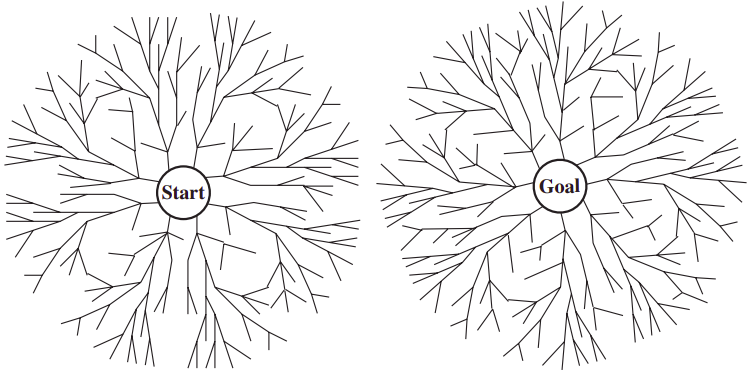
\includegraphics[
        width=\linewidth,
        height=4cm,
        keepaspectratio,
    ]{images/algorithms/bidirectional-search-illustration.png}
    \caption*{A schematic view of a bidirectional search that is about to succeed when a branch from the start node meets a branch from the goal node. \cite{ai/book/Artificial-Intelligence-A-Modern-Approach/Russell-Norvig}}
\end{figure}


\begin{enumerate}[itemsep=0.2cm]
    \item The idea behind bidirectional search is to run two simultaneous searches - one forward from the initial state and the other backward from the goal - hoping that the two searches meet in the middle
    \hfill \cite{ai/book/Artificial-Intelligence-A-Modern-Approach/Russell-Norvig}

    \item The motivation is that $b^{d/2} + b^{d/2}$ is much less than $b^d$
    \hfill \cite{ai/book/Artificial-Intelligence-A-Modern-Approach/Russell-Norvig}

    \item Bidirectional search is implemented by replacing the goal test with a check to see whether the frontiers of the two searches intersect; if they do, a solution has been found.
    \hfill \cite{ai/book/Artificial-Intelligence-A-Modern-Approach/Russell-Norvig}

    \item The check can be done when each node is generated or selected for expansion and, with a hash table, will take constant time.
    \hfill \cite{ai/book/Artificial-Intelligence-A-Modern-Approach/Russell-Norvig}

    \item \textbf{predecessors} of a state $x$ be all those states that have $x$ as a successor. Bidirectional search requires a method for computing predecessors. When all the actions in the state space are reversible, the predecessors of $x$ are just its successors. 
    \hfill \cite{ai/book/Artificial-Intelligence-A-Modern-Approach/Russell-Norvig}

    \item \textbf{Performance}:
    \begin{enumerate}
        \item \textbf{optimality}: 
        \begin{enumerate}
            \item YES \textbf{if} additional search is used to make sure the path isn’t another short-cut across the gap \textbf{else} NO
            \hfill \cite{ai/book/Artificial-Intelligence-A-Modern-Approach/Russell-Norvig}

            \item YES \textbf{if}  step costs are all identical \textbfit{and} both directions use breadth-first search \textbf{else} NO
            \hfill \cite{ai/book/Artificial-Intelligence-A-Modern-Approach/Russell-Norvig}
        \end{enumerate}

        \item \textbf{completeness}: YES \textbf{if} $b$ is finite \textbfit{and} both directions use breadth-first search \textbf{else} NO
        \hfill \cite{ai/book/Artificial-Intelligence-A-Modern-Approach/Russell-Norvig}

        \item \textbf{space complexity}:
        \begin{enumerate}
            \item using breadth-first searches in both directions: $\mathcal{O}(b^{d/2})$
            \hfill \cite{ai/book/Artificial-Intelligence-A-Modern-Approach/Russell-Norvig}
        \end{enumerate}

        \item \textbf{time complexity}:
        \begin{enumerate}
            \item using breadth-first searches in both directions: $\mathcal{O}(b^{d/2})$
            \hfill \cite{ai/book/Artificial-Intelligence-A-Modern-Approach/Russell-Norvig}
        \end{enumerate}
    \end{enumerate}
\end{enumerate}

























\section{Best-first search (BestFS) \cite{ai/book/Artificial-Intelligence-A-Modern-Approach/Russell-Norvig}}
\label{AI: Algorithms/Best-first search (BestFS)}


\begin{enumerate}
    \item Best-first search is an instance of the general \textsc{Tree-Search} or \textsc{Graph-Search} algorithm in which a node is selected for expansion based on an \textbf{evaluation function}, $f(n)$. $f(n)$ can be any function that returns a value for a given node.
    \hfill \cite{ai/book/Artificial-Intelligence-A-Modern-Approach/Russell-Norvig}

    \item The implementation of best-first graph search is identical to that for uniform-cost search, except for the use of $f$ instead of $g$ to order the priority queue.
    \hfill \cite{ai/book/Artificial-Intelligence-A-Modern-Approach/Russell-Norvig}

    \item Most best-first algorithms include $h$ as a component of $f$
    \hfill \cite{ai/book/Artificial-Intelligence-A-Modern-Approach/Russell-Norvig}
\end{enumerate}


\begin{lstlisting}[
    language=Python,
    caption=Problem Solving Agent - (General) Best-first search (BestFS) on a graph
]
def best_first_search(problem: Problem, f):
    node = Node(problem.initial_state, None, None, 0)

    if problem.goal_test(node.state):
        return solution(node)

    frontier = [(f(node), node)]
    heapq.heapify(frontier)
    explored = set()

    while frontier:
        _, node = heapq.heappop(frontier)

        if problem.goal_test(node.state):
            return solution(node)

        explored.add(node)

        for action in problem.actions(node.state):
            child = child_node(problem, node, action)
            if (all(n.state != child.state for n in explored) 
                and all(n.state != child.state for _, n in frontier)):
                heapq.heappush(frontier, (f(child), child))
            else:
                # Optional: Replace in frontier if better
                for i, (old_f, old_node) in enumerate(frontier):
                    if old_node.state == child.state and f(child) < old_f:
                        frontier[i] = (f(child), child)
                        heapq.heapify(frontier)
                        break

    return None
\end{lstlisting}







